\chapter{Hopfield Networks}
Questo tipo di rete è stata introdotta dal fisico, professore di chimica e biologia, John Hopfield nel 1982.



E' utilizzata per rappresentare \textbf{memoria indirizzabile del contenuto}: data una ragionevole porzione di informazione memorizzata, data una parziale o corrotta porzione, può essere completata recuperando ulteriori informazioni associate (la cosiddetta \textbf{pattern completion}). 


Il sistema preserva questa proprietà anche quando alcuni componenti sono inutilizzabili (\textbf{fault tollerance}).


Un esempio è il task di recuperare il paper chiamato \\
\textit{"H.A.KramersandG.H.Wannier,Phys.Rev.,60,252(1941)"}, cosa che si riesce a fare con \textit{"and Wannier(1941")} o addirittura con \textit{"Vannier(1941)"}.
\newline
\newline
Le \textbf{attractor networks} sono utili per memorizzare ricordi fondamentali che attraggono altri input. 



Il tipo dei ricordi che la rete memorizza è rappresentato dalla prima colonna dell'immagine che segue (quindi immagini parziali o corrotte), l'output è invece l'ultima colonna. Qundi la rete l'obiettivo della rete è capire che la prima immagine è un'immagine parziale di un ragno, che la seconda è un'immagine corrotta di due bottiglie e che la terza è di nuovo un'immagine parziale, ma di un cane.
\begin{figure}[!h]
    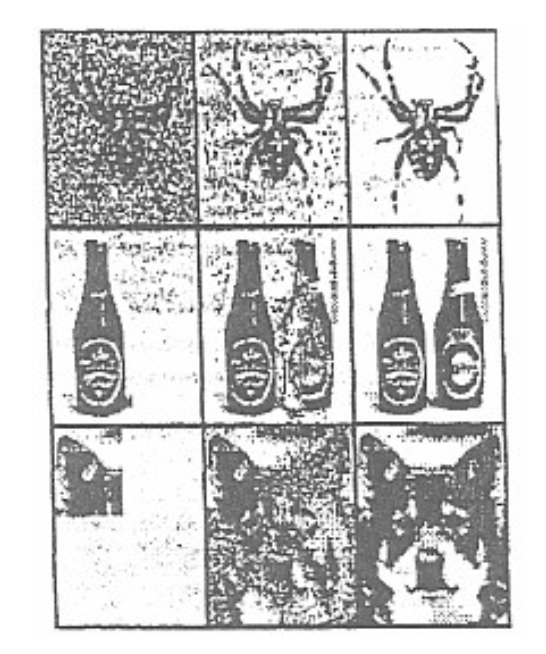
\includegraphics[scale=.5]{images/hopfield_networks/attr_net.png}
    \centering
\end{figure}

\newpage
La \textbf{pattern completion} caratterizza molta della nostra memoria, infatti, per esempio, il \textbf{riconoscimento di oggetti} (parzialmente nascosti) può essere visto come una sua instanza. Questa è una pratica che il cervello umano compie quotidianamente.
\begin{figure}[!h]
    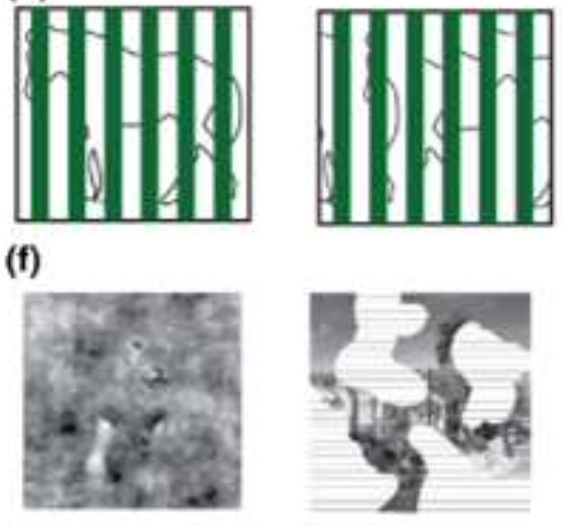
\includegraphics[scale=.5]{images/hopfield_networks/pattern_rec.png}
    \centering
\end{figure}

\section{Architettura}
In una Hopfield network \textbf{i neuroni di McCulloch-Pitts}  sono interconnessi ed ognuno di essi può avere due soli stati: $-1$ o $1$. Segue l'architettura della rete.
\begin{figure}[!h]
    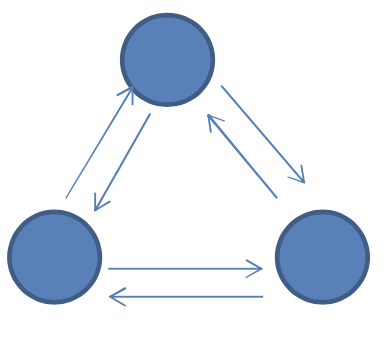
\includegraphics[scale=.7]{images/hopfield_networks/mp_net.png}
    \centering
\end{figure}



Date $N$ unità:
\begin{itemize}
    \item ogni neurone è connesso con tutti gli altri neuroni escluso se stesso;
    \item i pesi sono simmetrici: $w_{ij}=w_{ji}$.
\end{itemize}
\textbf{Nota:} questo esempio giocattolo, normalmente una rete di questo tipo è molto più grande di così.

\newpage
\subsection{Fase 1: Withdrawal/Retrieval Phase}
\textbf{In questa prima fase avviene la pattern completion}.



Stato di una rete con $N$ neuroni ad una data iterazione: attivazione degli $N$ neuroni $(1,- 1)$.
\begin{figure}[!h]
    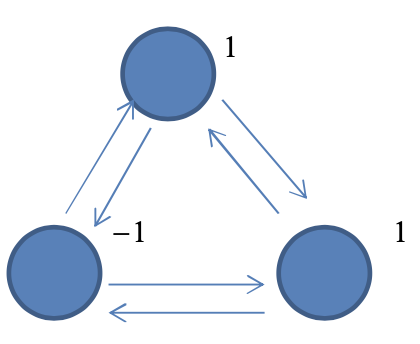
\includegraphics[scale=.7]{images/hopfield_networks/first_phase.png}
    \centering
\end{figure}



\textbf{L'input della rete} sono vettori di $1$ e $-1$ e di dimensione $N$. Ogni neurone rappresenta un elemento dell'input.



Quindi viene calcolata la nuova attivazione di un neurone alla volta scelto casualmente.



Questo procedimento continua finchè non sarà più possibile alcun cambiamento.
\newline
\newline
Il calcolo della nuova attivazione avviene compiendo i seguenti passi:
\begin{itemize}
    \item attivazione del $j-$esimo neurone alla $n-$esima iterazione: $n=y_j(n)\varphi(v_j(n))$;
    \item $v_j=$ net input per $j=\sum_{i=0}^Nw_{ji}y_i(n)$;
    \item $\varphi(v_j)(n)=
        \begin{cases}
            1                   & \text{se } v_j(n)>0)\\
            -1                  & \text{se } v_j(n)<0\\
            \varphi(v_j)(n-1)   & \text{se } v_j(n)=0\\
        \end{cases}$
\end{itemize}
\newpage
\subsection{Fase 2: Information Withdrawal}
\textbf{Input:} alla rete viene presentata una configurazione iniziale $x^*$ di $+1$ e $-1$ di lunghezza $N$. Per ogni neurone $j, y_j(0) = x^*(j)$.


\textbf{L'iterazione continua fino al raggiungimento della convergenza}. Nel processo, aggiorna gli elementi della rete in modo asincrono scegliendo un'unità a caso. La regola per aggiornare gli elementi è:
\begin{equation}
        y_j(n)=
        \begin{cases}
            1               & \text{se } \sum_{i=0}^Nw_{ji}y_i(n)>0\\
            -1              & \text{se } \sum_{i=0}^Nw_{ji}y_i(n)<0\\
            y_j(n-1)        & \text{se } v_j(n)=0\\
        \end{cases}
\end{equation}
\textbf{Convergenza:} si ripete l'operazione fino a trovare uno \textbf{stato stabile}, vale a dire per ogni unità $j$ abbiamo $y_j(n+1) = y_j(n)$.


\textbf{Output:} lo stato stabile trovato è l'output della rete.
\newline
\newline
Configurazione $-1,+1$:
\begin{figure}[!h]
    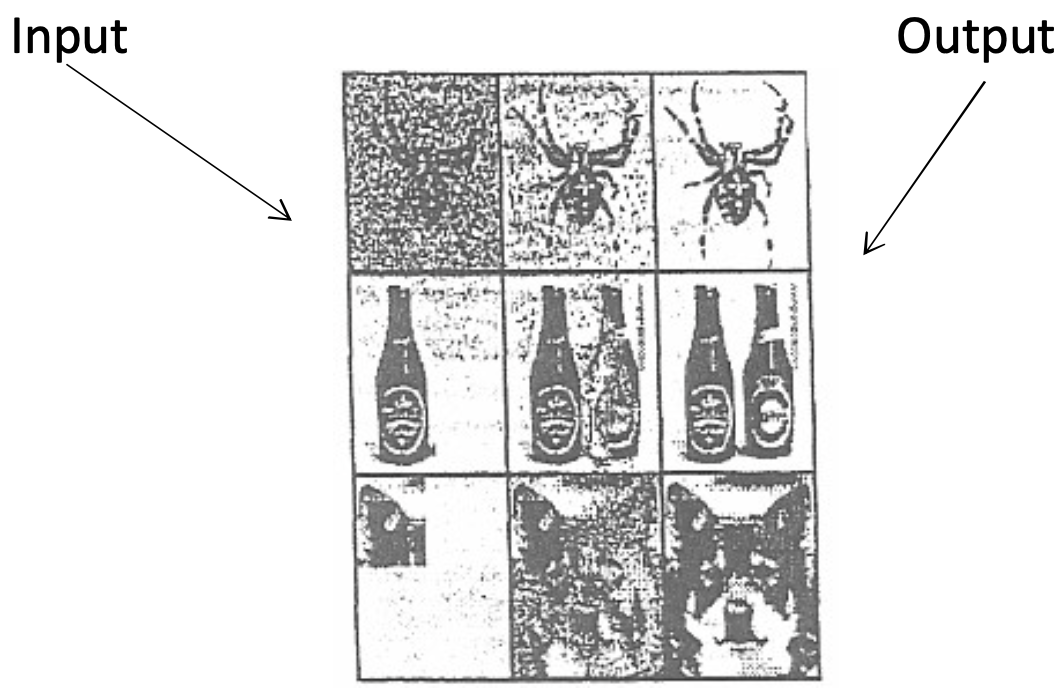
\includegraphics[scale=.35]{images/hopfield_networks/config.png}
    \centering
\end{figure}


Dato uno stato di partenza, gli stati attraverso i quali la rete passa, sono calcolati come segue: \textbf{le attivazioni dei neuroni sono calcolate in maniera asincrona}. Ogni volta che una unità viene scelta, la sua attività è calcolata attraverso le equazioni:
\begin{equation}
    v_j=\sum_{i=0}^Nw_{ji}y_i(n)
\end{equation}
\begin{equation}
    \varphi(v_j)(n)=
        \begin{cases}
            1                   & \text{se } v_j(n)>0)\\
            -1                  & \text{se } v_j(n)<0\\
            \varphi(v_j)(n-1)   & \text{se } v_j(n)=0\\
        \end{cases}
\end{equation}
\begin{figure}[!h]
    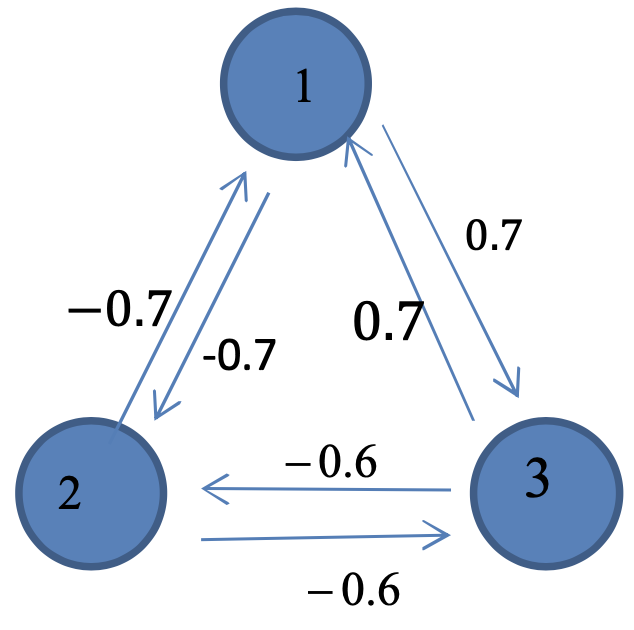
\includegraphics[scale=.35]{images/hopfield_networks/ex01.png}
    \centering
\end{figure}




In questo esempio la configurazione iniziale è $[-1,-1,1]$.
\begin{itemize}
    \item se scelgo $1$, $v_1=1.4=\phi(v_1)=1$ e ottengo $[1,-1,1]$;
    \item se scelgo $2$  $v_2=-1.3=\phi(v_2)=-1$ e ottengo $[1,-1,1]$;
    \item se scelgo $3$, rimane a $+1$.
\end{itemize}
$[1,-1,1]$ è uno stato stabile visto che $\forall i,y_i(n+1)=y_i(n)$.
\newpage
Nel seguente esempio, $[1,-1,1]$ è uno dei due stati stabili della rete, l'altro è $[-1,1,-1]$.
\begin{figure}[!h]
    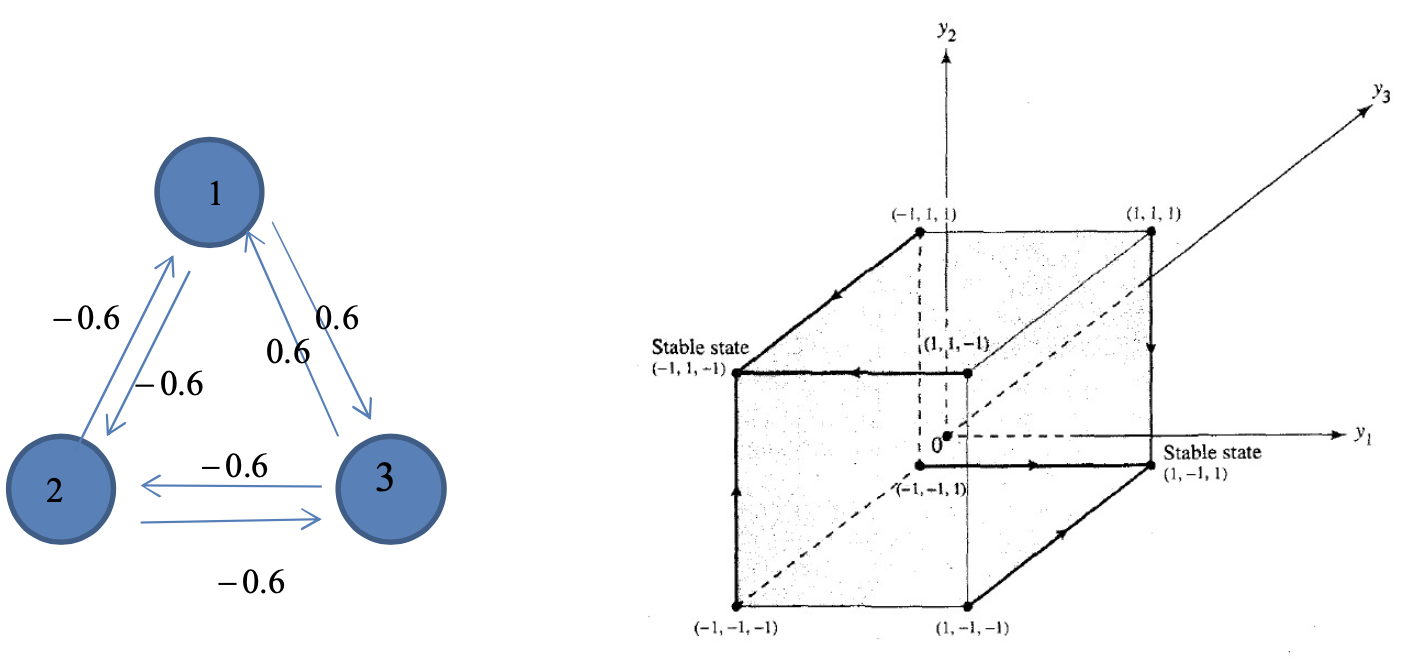
\includegraphics[scale=.5]{images/hopfield_networks/ex02.png}
    \centering
\end{figure}


I due stati stabili si comportano da \textbf{attrattori}: dato uno stato qualunque, esso convergerà ad uno dei due stati stabili.


Un \textbf{teorema di convergenza} garantisce che \textbf{dato uno stato di partenza, la rete giungerà sempre ad uno stato stabile}: le attività non potranno essere cambiate all'inifito.
\newline
\newline
In generale, \textbf{trovare uno stato stabile è un processo non deterministico}. Nel caso di reti con molte unità, potrebbero essere necessarie molte iterazioni.

\subsection{Fase 3: Storage Phase}
Come detto, le Hopfield Networks sono utilizzate per \textbf{memorizzare informazioni}. Ciò che vogliamo fare è memorizzare informazioni che lavorino come attrattori, stati stabili verso cui muovere gli altri stati.


Nel caso di memorizzazione di immagini, ci interessa:
\begin{itemize}
    \item l'immagine corrispondente allo stato stabile. Se la mostriamo alla rete, non si muove;
    \item se mostriamo alla rete una versione corrotta dell'immagine invece, essa convergerà all'immagine memorizzata.
\end{itemize}
Il problema, quindi, diventa \textbf{come creare l'informazione che vogliamo memorizzare}, i suoi ricordi fondamentali, gli stati stabili. Gli stati sono \textbf{resi stabili dai pesi}.
\newline
\newline
Dati $M$ vettori di ricordi fondamentali $f_1,f_2,\dots$ di dimensione $N$, li memorizziamo nel seguente modo:
\begin{equation}
    w_{ji}=\frac{1}{M}\sum^M_{k=1}f_k(i)\bullet f_k(j) \text{ se } j\neq i.
\end{equation}
Per ogni ricordo fondamentale prodotto tra l'$i-$esimo e il $j-$esimo elemento:
\begin{itemize}
    \item se essi hanno segno concorde, $f(i)\bullet f_k(j)>0$, contribuirà a rafforzare $w_{ji}$;
    \item se hanno segno discorde, contribuirà a indebolire $w_{ji}$.
\end{itemize}
\newpage
Dato un set di \textbf{fundamental memories}, dobbiamo trovare i pesi adeguati. L'algoritmo di apprendimento si basa sul \textbf{principio di Hebb}:
\begin{itemize}
    \item rafforzamento delle connessioni tra unità con la stessa attivazione;
    \item indebolimento delle connessioni tra unità con attivazioni opposte.
\end{itemize}


\textbf{Il principio di Hebb ha anche una controparte neurobiologica}: le sinapsi tra unità che sono spesso attive allo stesso tempo vengono rafforzate, mentre le sinapsi tra neuroni che non sono attivi simultanemanete vengono indebolite.


I neuroni che si attivano insieme si collegano insieme.
\begin{figure}[!h]
    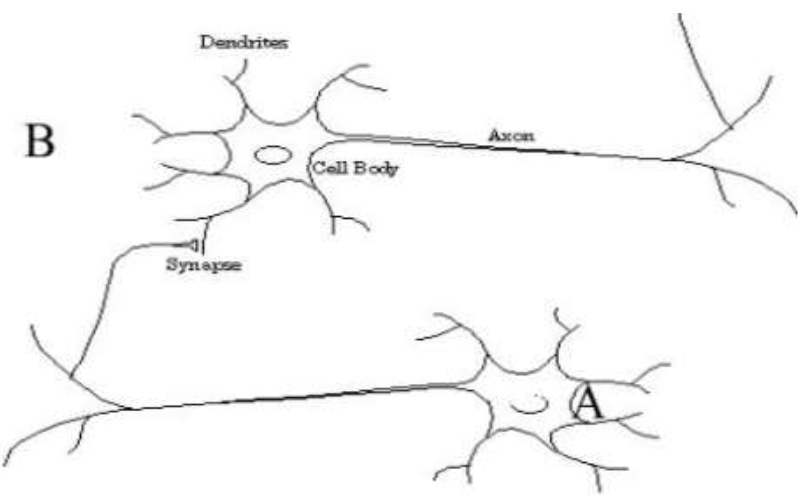
\includegraphics[scale=.5]{images/hopfield_networks/neurons.png}
    \centering
\end{figure}



\textbf{Nota:} seguendo la tradizione, abbiamo presentato prima la \textbf{withdrawal phase} e poi la \textbf{storage phase}. Tuttavia, cronologicamente, avvengonono nell'ordine inverso.

\section{Esercizio}
Applicare la regola sapendo che $[1,-1,1]$ e $[-1,1,-1]$ sono stati stabili: essi sono le fundamental memories da memorizzare.
\begin{equation}
    w_{ji}=\frac{1}{M}\sum^M_{k=1}f(i)\bullet f_k(j) \text{ se } j\neq i.
\end{equation}
\begin{figure}[!h]
    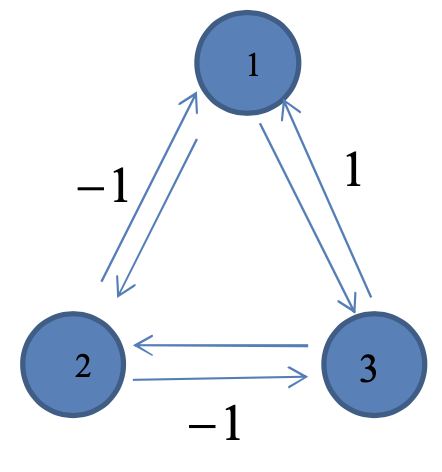
\includegraphics[scale=.5]{images/hopfield_networks/ex03.png}
    \centering
\end{figure}


Soluzione:
\begin{equation}
    \begin{split}
        w_{21}=w_{12}=\frac{1}{2}\sum^2_{k=1}f_k(1)\bullet f_k(2) = \frac{1}{2}\Big( 1\bullet(-1)+(-1)\bullet 1) \Big) = -1 \\
        w_{23}=w_{32}=\frac{1}{2}\sum^2_{k=1}f_k(2)\bullet f_k(3) = \frac{1}{2}\Big( 1\bullet(-1)+(-1)\bullet 1) \Big) = -1 \\
        w_{31}=w_{13}=\frac{1}{2}\sum^2_{k=1}f_k(1)\bullet f_k(3) = \frac{1}{2}\Big( 1\bullet1+(-1)\bullet (-1)) \Big) = 1
    \end{split}
\end{equation}
\newpage

\section{Il teorema di convergenza}
\textbf{Teorema:} dato uno stato qualunque della rete, la rete converge ad uno stato stabile.
\begin{itemize}
    \item Date $N$ unità, abbiamo $2^N$ possibili stati per la rete;
    \item ad ognuno di questi stati è associato un \textbf{energy value};
    \item dimostriamo che ogni cambiamento di stato della rete porta ad un abbassamento dell'energy value;
    \item c'è un momento nel quale non ci sono stati raggiungibili che abbiamo \textbf{energy value minore}.
\end{itemize}


\textbf{Energy Function}:
\begin{equation}
    E=-\frac{1}{2}\sum_i\sum_jw_{ij}y_iy_j.
\end{equation}
L'energia $E$ \textbf{misura la propensione della rete a cambiare stato (opposto dell'armonia)}, è infatti una misura \textit{cattiva}.


Dimostriamo che ogni cambiamento nello stato diminuisce $E$.



\textbf{Nota:} grossomodo, \textbf{harmony} aumenta con il numero di $w_{ij}y_iy_j$ positivi: 
\begin{itemize}
    \item \textbf{higher harmony} $=$ \textbf{meno propensione al cambiamento dello stato};
    \item  \textbf{lower harmony} $=$ \textbf{più propensione al cambiamento dello stato}.
\end{itemize}


Ogni prodotto $w_{ij}y_iy_j$ \textbf{è positivo se $y_i$ e $y_j$ hanno segno concorde e $w_{ij}$ è positivo ed è negativo se hanno segno discorde e $w_{ij}$ è negativo}.


Esempio:
\begin{figure}[!h]
    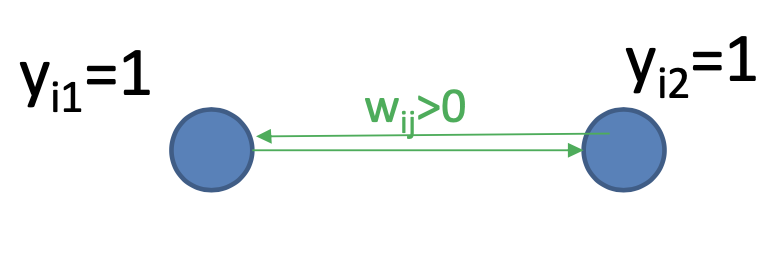
\includegraphics[scale=.5]{images/hopfield_networks/ex04.png}
    \centering
\end{figure}


Intuitivamente, la rete in questo esempio è instabile. Ha alta energia quindi alta propensione al cambiamento.
\newline
\newline
Consideriamo ora come cambia $E$ rispetto al cambio di attivazione della $k-$esima unità. $E$ ed $E'$ denotano l'energia prima e dopo il cambiamento di $y_k$:
\begin{equation}
    \begin{split}
        E=-\frac{1}{2}\sum_i\sum_jw_{ij}y_iy_j =-\frac{1}{2}\Big( \sum_{i\neq k}\sum_{j\neq k}w_{ij}y_iy_j + 2 \sum_{j\neq k}w_{kj}y_ky_j \Big)\\
        E'=-\frac{1}{2}\Big( \sum_{i\neq k}\sum_{j\neq k}w_{ij}y_iy_j + 2 \sum_{j\neq k}w_{kj}y'_ky_j \Big)\\
        E-E'=-\frac{1}{2}\Big(\Big(2\sum_{j\neq k}w_{kj}y_ky_j-2\sum_{j\neq k} w_{kj}y'_ky_j\Big)\Big)=-\sum_{j\neq k}w_{kj}y_j(y_k-y'_k).
    \end{split}
\end{equation}
\newpage
Innanzitutto notiamo che  $v_k=\sum_{j\neq k}w_{kj}y_j$.


Proseguendo, distinguiamo due casi:
\begin{itemize}
    \item $y_k$ passa da $+1$ a $-1$, quindi $y_k-y'_k>0$ e $\sum_jw_{kj}y_j<0$:
        \begin{equation}
            -\sum_{j\neq k}w_{kj}y_j(y_k-y'_k)>0\text{ e }E>E';
        \end{equation}
    \item $y_k$ passa da $-1$ a $+1$, quindi $y_k-y'_k>0$ e $\sum_jw_{kj}y_j>0$ quindi di nuovo:
        \begin{equation}
            -\sum_{j\neq k}w_{kj}y_j(y_k-y'_k)>0\text{ e }E>E'.
        \end{equation}
\end{itemize}
\textbf{Ad ogni cambiamento $E$ diminuisce}. Visto che gli stati sono finiti, ad un dato punto arriveremo ad uno stato che non cambia: \textbf{uno stato stabile}.
\begin{figure}[!h]
    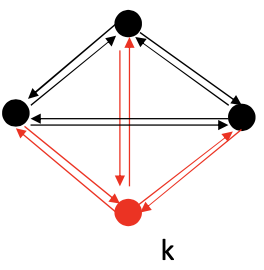
\includegraphics[scale=2]{images/hopfield_networks/conv_theorem.png}
    \centering
\end{figure}
\newpage
\section{Conclusioni}
\subsection{Punti forti}
\begin{itemize}
    \item \textbf{Completano pattern parziali};
    \item  \textbf{generalizano}, dato un input simile a quello che è stato memorizzato, recuperano l'informazione corrispondente;
    \item sono \textbf{fault tolerant}, se qualche sinapsi si rompe (brain damage) l'output rimane ragionevole;
    \item permettono \textbf{l'estrazione di prototipi}, se la rete impara molte informazioni simili tra di esse, crea il loro prototipo e questo diventa lo stato presentato esplicitamente;
    \item la regola di apprendimento apprendimento è \textbf{Hebb like}, la quale è biologicamente plausibile e ci sono provo della sua esistenza nel cervello;
    \item può tenere conto degli \textbf{effetti del contesto}, noi ricordiamo meglio ciò che impariamo se siamo messi nello stesso contesto
\end{itemize}
\subsection{Punti deboli}
Sfortunatamente, non tutti gli stati stabili sono fundamental memories memorizzati durante lo storage. Esistono i cosiddetti \textbf{stati spuri}:
\begin{itemize}
    \item l'opposto di uno stato stabile è ancora uno stato stabile;
    \item la combinazione di stati stabili è ancora uno stato stabile.
\end{itemize}
La capacità di storage con degli errori data da $N$ unità è di $0.14N$.
Altri lati negativi sono:
\begin{itemize}
    \item capacità di storage limitata;
    \item errori;
    \item nel cervello le sinapsi non sono simmatriche;
    \item nel cervello non ci sono stati stabili, ma solo stati transitori i quali evolvono in stati successivi. Esistono delle estensioni delle Hopfield Networks che imparano sequenze di stati.
\end{itemize}
\subsection{Modelli ibridi}
Alcuni ricercatori utilizzando oggi \textbf{modelli ibridi}.

